% !TEX program = xelatex
% 中文版 —— 编译方式：XeLaTeX（需 ctex 宏包支持中文）
% Overleaf 使用：上传本文件，Menu → Settings → Compiler → 选 XeLaTeX
\documentclass[11pt,a4paper]{ctexart}

\usepackage[utf8]{inputenc}
\usepackage{amsmath,amssymb}
\usepackage{booktabs}
\usepackage{array}
\usepackage{graphicx}
\usepackage{hyperref}
\usepackage[margin=2.5cm]{geometry}
\usepackage{enumitem}
\usepackage{url}

\hypersetup{colorlinks=true, linkcolor=blue, citecolor=blue, urlcolor=blue}

\title{\textbf{基于子答案双向交叉核验的图约束多跳推理方法}}
\author{Anonymous Authors}
\date{}

\begin{document}
\maketitle

% ===== 摘要 =====
\begin{abstract}
\noindent
部分图结构增强推理变体使用纯图论结构指标（连通性、无环性、覆盖度）作为一致性校验，但这类指标不一定反映推理内容正确性。在本文的结构分变体中，Consistency Score 几乎不具备对错区分能力，多路选优退化为近似随机抽取。本文提出 GERS，将推理显式建模为推理依赖图（DAG）并按拓扑序执行；核心创新是\textbf{子答案双向交叉核验}：以最终答案与上下文为锚，反向逐个重答子问题，对比正反向子答案一致性，将 Consistency Score 从结构合法性指标升级为内容自洽信号。在 HotpotQA 500 条上，该方法将对错区分度从 $-0.0035$ 修复到 $+0.0847$，AUROC 从 0.498 提升到约 0.58--0.59；点估计最高配置 GERS-CV2 取得 EM=0.302、F1=0.413，相比 CoT-SC 的 F1 高 4pt，EM 对错的 McNemar 检验显著（$p=0.029$），但配对 bootstrap 效应量区间仍微跨零。本文同时明确指出自洽不等于正确：许多高 CS 答案仍然错误，2WikiMultiHopQA 也暴露了深桥接对比题上的错误传播边界。
\end{abstract}

\noindent\textbf{关键词：} 大语言模型；多跳推理；思维链；图结构表征；双向交叉核验；一致性诊断

% ===== 1 引言 =====
\section{引言}

多跳推理（multi-hop reasoning）要求模型跨多个证据片段组合推导出答案，是衡量大语言模型（LLM）复杂推理能力的核心任务之一。Chain-of-Thought（CoT）提示~\cite{wei2022cot} 通过引导模型输出中间推理步骤，显著提升了 LLM 在此类任务上的表现。然而，标准 CoT 以\textbf{线性文本}串接推理步骤，存在两类核心不足：

\begin{enumerate}[label=\arabic*.]
\item \textbf{非线性依赖缺失}：CoT 以线性文本串接推理步骤，无法表达子问题间的分支、合流与并行依赖。当推理路径本应是有向无环图（DAG）而非链时——例如``对比型''问题需要先分别求解两条子链再汇合比较——线性化会导致结构信息丢失，模型易在汇合点出错。
\item \textbf{质量无差别投票}：CoT-SC~\cite{wang2023sc} 通过多次采样取众数答案提升稳健性，但其投票是``等权''的——每条候选推理路径无论结构完整性如何都计一票，无法利用推理路径本身的质量信息。
\end{enumerate}

近期工作尝试用图结构增强推理：GoT~\cite{besta2024got} 提出思维图支持合并与蒸馏，但不采用本文的子问题拓扑执行；RwG~\cite{han2025rwg} 将上下文隐式知识结构化为实体关系图；MoDeGraph~\cite{oruche2025modegraph} 引导 LLM 提取实体关系构建多跳依赖图，属于 prompt 方法。GERS 关注当图结构参与子问题执行与校验时，图派生一致性分数是否能作为诊断与弱候选质量信号。

针对上述问题，本文提出 \textbf{GERS}（Graph-Enhanced Reasoning System），将推理显式建模为推理依赖图（DAG）并按拓扑序执行。我们发现，单纯用图论结构性质（连通性、无环性、覆盖度）计算 Consistency Score 是无效的——LLM 生成的分解图几乎都是合法 DAG，导致所有样本得分趋同（聚集在 0.6$\sim$0.7），多路选优退化为随机抽取（500 条实测对错区分度仅 $-0.0035$）。为此，本文提出核心创新\textbf{子答案双向交叉核验}：以最终答案 + 上下文为锚，反向逐个重答每个子问题，对比正向子答案与反向子答案的一致性，将 Consistency Score 从``图是否合法''升级为``推理内容是否自洽''。这一机制由显式 DAG 分解自然支持；线性 CoT 没有可独立核验的子问题结构，难以直接应用同类核验。

本文不声称图约束推理在所有多跳任务上全面超越 CoT，而是指出图推理方法中一个被忽视的问题：图结构合法性并不等于推理内容正确性。贡献分三层：
\begin{enumerate}[label=\arabic*.]
\item \textbf{机制贡献（核心）}：子答案双向交叉核验将 Consistency Score 的对错区分度从 $-0.0035$ 修复到 $+0.0847$，AUROC 从 0.498 提升到约 0.58--0.59（500 条 HotpotQA），使一致性校验从结构指标升级为弱但有用的内容自洽诊断信号。该核验由显式 DAG 分解自然支持。
\item \textbf{经验贡献}：点估计最高配置 GERS-CV2 在 HotpotQA 500 条上取得 EM=0.302、F1=0.413，相比 CoT-SC 的 F1 高 4pt，且 EM 对错的 McNemar 检验显著（$p=0.029$），但配对 bootstrap 效应量区间仍微跨零，本文如实报告。
\item \textbf{诊断贡献}：在 2WikiMultiHopQA 上给出边界分析，方法适用于对比型分解，但在深桥接对比题上因上游实体错误传播而失效；并报告当前测试的旧结构分图级多路选优在中等难度多跳上无额外增益。
\end{enumerate}

% ===== 2 相关工作 =====
\section{相关工作}

\noindent\textbf{思维链推理。}Wei 等~\cite{wei2022cot} 提出 Chain-of-Thought prompting。Wang 等~\cite{wang2023sc} 提出 Self-Consistency（CoT-SC），通过多次采样取众数答案提升稳健性，但其等权投票未利用推理路径质量。Yao 等~\cite{yao2023tot} 提出 Tree of Thoughts（ToT），以树搜索框架支持状态评估与回溯，但子问题间无显式依赖建模。这些方法均基于线性或树形结构，未显式建模子问题间的依赖图。

\noindent\textbf{图结构增强推理。}GoT~\cite{besta2024got} 将推理建模为图，支持合并、蒸馏等操作，但侧重 Prompt 工程而非执行约束。RwG~\cite{han2025rwg} 通过 LLM 在上下文中构建实体关系图。MoDeGraph~\cite{oruche2025modegraph} 引导 LLM 构建多跳依赖图辅助多跳问答，但本质仍是 prompt 方法。与这些工作不同，GERS 将推理依赖图与执行流程耦合，并研究图派生一致性作为诊断与弱排序信号的作用。

\noindent\textbf{一致性校验与自评估。}Process Reward Models~\cite{lightman2024verify} 通过对中间步骤打分进行过程监督，但依赖大量标注数据。Self-Refine~\cite{madaan2023selfrefine} 通过自我反馈迭代修正答案，但作用于线性文本、无可核验的子问题结构。GERS 采用图论算法进行结构化校验，并在此基础上设计子答案双向交叉核验，使一致性分数可被分析并用于受控变体。

\begin{table}[h]
\centering
\caption{GERS 与代表性推理范式的定位对比。该表用于澄清适用范围，不表示对所有方法的全面经验优势。}
\small
\begin{tabular}{lccc}
\toprule
方法族 & 结构 & 执行顺序 & 可核验子答案 \\
\midrule
CoT & 线性文本 & 隐式 & 否 \\
CoT-SC & 多条线性样本 & 隐式 & 否 \\
ToT / GoT & 树或图状 thought & 搜索/灵活 & 状态或 thought 节点 \\
RwG / 图提示 & 实体/上下文图 & prompt 条件化 & 通常否 \\
MoDeGraph-style & 依赖图 prompt & prompt 条件化 & 实体/关系级 \\
GERS & 子问题 DAG & 拓扑执行 & 是，正反向核验 \\
\bottomrule
\end{tabular}
\end{table}

% ===== 3 方法 =====
\section{方法}

\subsection{总体框架}

GERS 的推理流程分为推理状态图表示、图约束链路生成与一致性校验三个模块，如图~1 所示：输入问题 $Q$ 与上下文 $C$ $\to$ ① LLM 将 $Q$ 分解为子问题 $\{q_i\}$ 及依赖关系 $\to$ ② 构建推理 DAG $G=(V,E)$，Fact$(Q) \to$ Step$(q_i) \to$ Conclusion $\to$ ③ 拓扑排序 $\tau = \text{topo\_sort}(G)$ $\to$ ④ 按拓扑序逐步执行，注入前驱答案生成 $a_i$ $\to$ ⑤ 汇总推理链生成最终答案 $A$（答案类型回扣） $\to$ ⑥ 计算交叉验证一致性分 $S = \alpha \cdot S_{\text{struct}} + \beta \cdot S_{\text{crossval}}$ $\to$ 输出答案 $A$ + 推理图 $G$ + Score $S$。另设历史诊断基线 GERS-SC：采样 K 条 DAG 并用原始结构 CS 选优。

\begin{figure}[h]
\centering
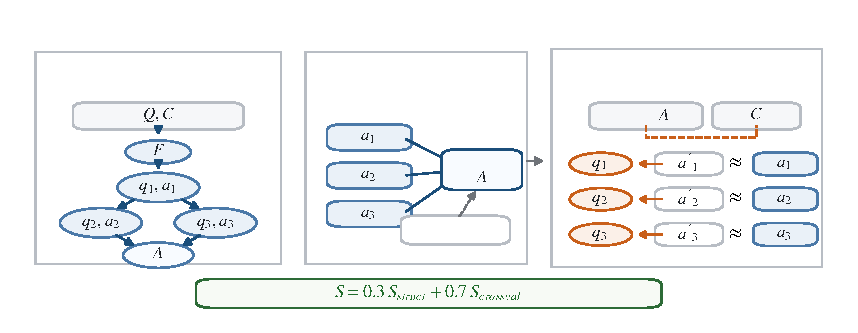
\includegraphics[width=0.85\textwidth]{figures/image1}
\caption{GERS 推理框架。}
\end{figure}

\subsection{推理状态图表示}

推理图 $G=(V,E)$ 的节点类型包括：FactNode（事实节点，已知信息/原始问题）、StepNode（过程节点，子问题及答案）、ConclusionNode（目标节点，最终结论）。边类型包括：DeriveEdge（推导边 $u \to v$）、SupportEdge（支撑边）、ConflictEdge（互斥边）。构建过程：LLM 将问题 $Q$ 分解为有序子问题列表 $\{q_1, \dots, q_n\}$，每个子问题标注依赖关系，据此创建节点与 DeriveEdge。

\subsection{图约束链路生成}

\textbf{路径规划。}对推理图 $G$ 执行拓扑排序，得到执行顺序 $\tau = (v_1, \dots, v_n)$。若存在环路则破环后排序。拓扑序确保每个子问题被回答时其所有前驱已获得答案。

\textbf{逐步执行与汇总。}按拓扑序逐个调用 LLM 回答子问题，每个子问题答案作为后续依赖子问题的上下文（依赖传递）。全部回答后汇总推理链生成最终答案 $A$。

\textbf{答案类型回扣。}汇总阶段约束最终答案必须匹配原始问题要求的实体类型（如问``which film''则答案须为电影名而非中间实体导演名），对复合桥接题的答案对齐至关重要。

\subsection{一致性校验与子答案双向交叉核验}

\textbf{结构层 Consistency Score（基线）。}GERS 首先计算纯图论结构得分：
\begin{equation}
S_{\text{struct}} = w_1 \cdot C_{\text{conn}} + w_2 \cdot C_{\text{cycle}} + w_3 \cdot C_{\text{cov}}
\end{equation}
其中 $w_1=w_3=0.35, w_2=0.30$，分别为连通性、无环性、覆盖度，并引入推理链长度惩罚。

\textbf{结构层的局限。}实测发现，LLM 生成的分解图几乎都是合法连通无环 DAG，导致 $S_{\text{struct}}$ 高度聚集（500 条均值 0.662，标准差 0.098，对错区分度 $-0.0035$），完全无法区分推理好坏。

\textbf{子答案双向交叉核验（核心创新）。}给定正向子答案 $\{a_i\}$ 与最终答案 $A$，以``最终答案 $A$ + 上下文 $C$''为锚反向逐个重答子问题，得反向子答案 $\{a'_i\}$，对比一致性：

\begin{figure}[h]
\centering
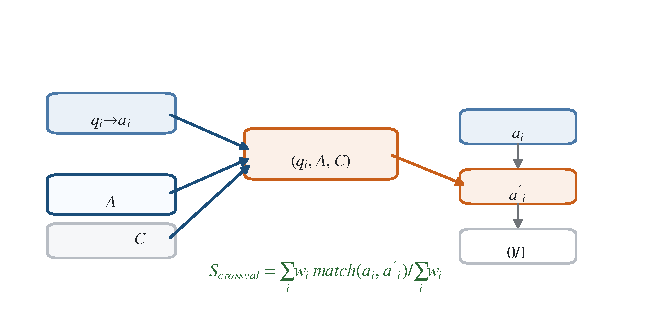
\includegraphics[width=0.85\textwidth]{figures/image3}
\caption{双向交叉核验机制示意图。}
\end{figure}
\begin{equation}
S_{\text{crossval}} = \frac{\sum_{i=1}^{n} w_i \cdot \mathbb{1}[\text{match}(a_i, a'_i)]}{\sum_{i=1}^{n} w_i}
\end{equation}
其中权重 $w_i = 0.5 + 0.5\cdot(i+1)/n$ 使下游子问题（拓扑序靠后）权重更高，因其错误传播更远。$\text{match}$ 为三级启发式：(i) 归一化后精确匹配（小写、去标点、yes/no 与数值统一）返回 1；(ii) 包含关系或数值相等返回 1；(iii) 否则 0。可启用 LLM 判断（默认关闭以控成本）处理残余语义情形。反向重答 Prompt 显式要求``基于上下文独立重答，勿照抄最终答案''，缓解 confirmation bias。该交叉核验由显式 DAG 分解（提供命名子问题单元与依赖边）自然支持，比应用于非结构化 CoT 文本更直接、更可解释。

\textbf{confirmation bias 控制。}由于反向验证默认可见最终答案 $A$，我们额外评测仅使用上下文、不使用答案锚点的反向验证变体。该变体得到 EM 0.300 / F1 0.414，CS 降至 0.646；默认设置为 EM 0.302 / F1 0.413 / CS 0.777。端任务结果基本不变，说明收益并非简单来自把最终答案喂回模型；但 CS 降低也说明答案锚点确实会提高内部一致性，不能把 CS 解释为事实正确性概率。

\textbf{新 Consistency Score。}
\begin{equation}
S = 0.3 \cdot S_{\text{struct}} + 0.7 \cdot S_{\text{crossval}}
\end{equation}

\subsection{子答案置信度加权汇总}

每个子答案置信度由轻量启发式估计（零额外 LLM 调用），综合考量答案非空、不含不确定信号、核心实体在上下文落地、是否纯数字。低于阈值 $\theta_{\text{conf}}=0.5$ 的子答案在汇总 Prompt 中标注 \texttt{[LOW CONFIDENCE]}，降低单步错误向最终答案的传播。

\subsection{图级自一致性（GERS-SC）}

GERS-SC 生成 K 条不同推理 DAG（分解温度 $T \in \{0.3, 0.5, 0.7\}$），用 Consistency Score 选得分最高者：$A^* = \arg\max_{k} S(G_k)$。主表中评测的 GERS-SC 使用原始结构分进行选优；其失效正是双向交叉验证的动机。是否用新的 cross-validated score 扩展到完整 K 路选优，由于会进一步放大验证成本，留作未来工作。

% ===== 4 实验 =====
\section{实验}

\subsection{实验设置}

\textbf{数据集。}HotpotQA~\cite{yang2018hotpotqa}（500 条，bridge 404 + comparison 96）作为主实验；2WikiMultiHopQA~\cite{ho20202wiki} 作为边界分析，包括 100 条分题型诊断集与 300 条扩展检查。

\textbf{基线方法。}Zero-Shot、Standard CoT、CoT-SC（$N=3$）、CoT-SC+GERS 重排（消融对照）以及 MoDeGraph-style 图提示基线。MoDeGraph-style 基线是依据公开方法描述实现的非官方版本，并非官方代码复现。所有方法采用统一的简洁答案提取与归一化流程。

\textbf{本文方法。}GERS+自适应（DAG 执行 + 自适应路由）；GERS-SC（+图级自一致性 K=3）；GERS-CV（+双向交叉验证）；GERS-CV2（+置信度加权汇总，点估计最高配置）。

\textbf{模型与配置。}Qwen3-8B（DashScope API），多线程并行（4 worker），零失败。\textbf{评估指标：}EM、F1、Consistency Score。主对比报告 EM/F1 差值的配对 bootstrap 95\% CI（10000 次重采样），并对 EM 对错进行配对 McNemar 检验。

\textbf{评估公平性。}为降低评估链路缺陷扭曲对比的风险，本文统一三项处理：(1) 修复 EM 双向子串匹配 bug（原会使数值答案虚高）；(2) 所有方法使用同一套简洁答案提取与归一化代码；(3) GERS 汇总阶段加入答案类型回扣，因为 DAG 执行可能输出中间实体而非最终问题要求的实体。这些控制降低但不能完全消除 prompt 格式差异对比较的影响。

\subsection{主实验结果}

\begin{figure}[h]
\centering
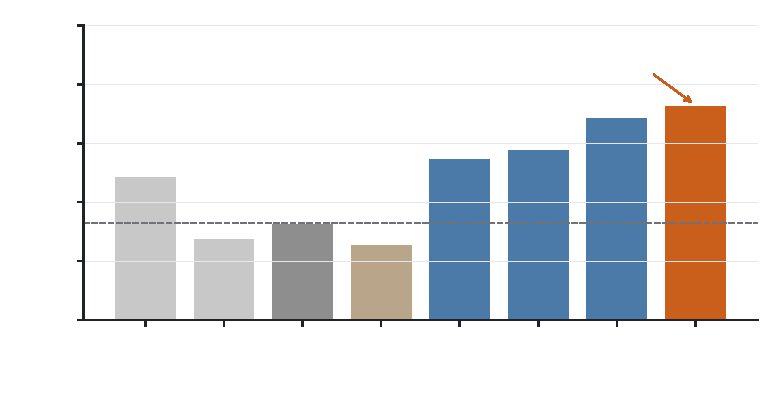
\includegraphics[width=0.85\textwidth]{figures/image4}
\caption{HotpotQA 主实验 F1 对比（n=500）。图中标注的是 GERS-CV2 相对 CoT-SC 的 F1 差值及配对 bootstrap 区间。}
\end{figure}

\begin{table}[h]
\centering
\caption{主实验结果（HotpotQA, n=500）}
\begin{tabular}{lccc}
\toprule
方法 & EM & F1 & CS \\
\midrule
Zero-Shot & 0.276 & 0.389 & — \\
Standard CoT & 0.264 & 0.368 & — \\
CoT-SC (N=3) & 0.262 & 0.373 & — \\
CoT-SC+GERS 重排 & 0.264 & 0.372 & — \\
MoDeGraph-style prompt & 0.252 & 0.366 & — \\
GERS+自适应 & 0.284 & 0.395 & 0.996 \\
GERS-SC (K=3) & 0.282 & 0.398 & 0.662 \\
GERS-CV（+双向交叉验证） & 0.298 & 0.409 & 0.782 \\
\textbf{GERS-CV2（+置信度加权）} & \textbf{0.302} & \textbf{0.413} & 0.777 \\
\bottomrule
\end{tabular}
\end{table}

GERS-CV2 取得点估计最高 EM=0.302、F1=0.413，相比 CoT-SC EM +4pt、F1 +4pt，且 EM 对错的 McNemar 检验达到配对显著。它也高于本文非官方 MoDeGraph-style 图提示基线（F1 0.366），说明该 prompt-only 图实现是当前设置下的较弱基线，但不能外推到官方 MoDeGraph 或所有图推理系统。双向交叉验证（GERS+自适应 0.284 $\to$ GERS-CV 0.298）带来 +1.4pt EM 增益，是本文核心创新的直接贡献。HotpotQA 上 Zero-Shot（0.276）已接近 GERS——该数据集上下文直接包含答案证据，压缩了所有``高级''方法的优势空间；CoT-SC 甚至低于 Zero-Shot。

\begin{table}[h]
\centering
\caption{显著性检验（HotpotQA, n=500）。EM/F1 差值报告配对 bootstrap 95\% CI；McNemar $p$ 基于 EM 对错。}
\begin{tabular}{lccccc}
\toprule
对比 & EM差值 & EM 95\% CI & F1差值 & F1 95\% CI & McNemar $p$ \\
\midrule
GERS-CV2 vs CoT-SC & +0.040 & [$-0.014, +0.096$] & +0.041 & [$-0.014, +0.095$] & \textbf{0.029} \\
GERS-CV2 vs Standard CoT & +0.038 & [$-0.018, +0.094$] & +0.045 & [$-0.009, +0.099$] & \textbf{0.040} \\
GERS-SC vs CoT-SC & +0.020 & [$-0.034, +0.076$] & +0.025 & [$-0.029, +0.079$] & 0.275 \\
\bottomrule
\end{tabular}
\end{table}

GERS-CV2 在 EM 对错的 McNemar 配对检验下显著优于 CoT-SC（$p=0.029$），但 EM 与 F1 的配对 bootstrap 95\% CI 均微跨零（下限约 $-0.014$）。本文如实报告这一``对错配对显著、效应量临界''状态。相比之下，未引入双向交叉核验的 GERS-SC（$p=0.275$）不显著，与核心机制的贡献方向一致。

\subsection{Consistency Score 区分度的修复（核心证据）}

\begin{figure}[h]
\centering
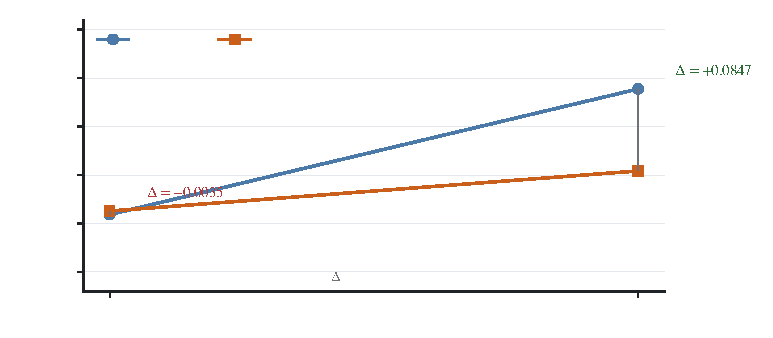
\includegraphics[width=0.8\textwidth]{figures/image2}
\caption{Consistency Score 区分度对比：旧 CS（纯结构）与新 CS（+双向交叉验证）。}
\end{figure}

\begin{table}[h]
\centering
\caption{Consistency Score 对错区分度（HotpotQA, n=500）}
\begin{tabular}{lcccc}
\toprule
CS 计算方式 & 答对 CS 均值 & 答错 CS 均值 & 区分度 & 分布 stdev \\
\midrule
旧 CS（纯结构，GERS-SC） & 0.6592 & 0.6628 & $\mathbf{-0.0035}$ & 0.098 \\
新 CS（+双向交叉验证，GERS-CV） & 0.7888 & 0.7042 & $\mathbf{+0.0847}$ & 0.340 \\
对照：纯结构分 $S_{\text{struct}}$ & 0.9967 & 1.0000 & $-0.0033$ & — \\
\bottomrule
\end{tabular}
\end{table}

旧 CS 几乎无区分能力：纯图论结构指标区分度为 $-0.0035$（反向），分布高度聚集（stdev 0.098）。双向验证修复了信号方向与幅度：新 CS 区分度跃升至 $+0.0847$，分布拉开（stdev 0.340）。但该信号仍不等同于正确性验证器；它更适合作为弱排序/诊断信号。以 EM 对错为标签，旧结构 CS 的 AUROC 为 0.498，GERS-CV 为 0.581，GERS-CV2 为 0.589。GERS-CV2 中 250 条样本得到 CS=1.0，但其中 156 条仍为 EM 错误，说明内部自洽并不保证事实正确。

\subsection{分题型分析与适用边界}

\begin{figure}[h]
\centering
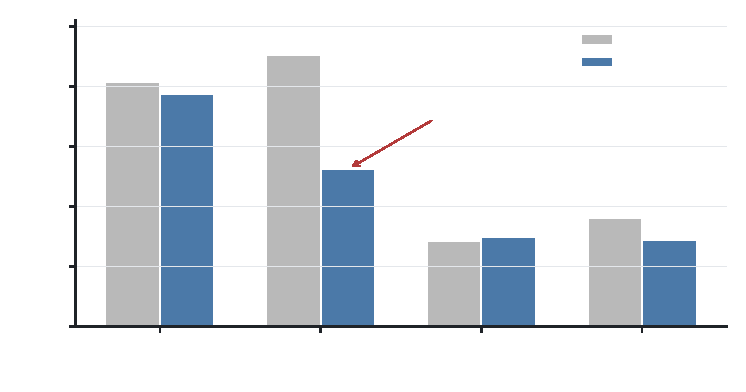
\includegraphics[width=0.85\textwidth]{figures/image5}
\caption{2WikiMultiHopQA 分题型 F1 对比（诊断性实验，n=100）。横轴标出各题型样本数。}
\end{figure}

\begin{table}[h]
\centering
\caption{2WikiMultiHopQA 分题型 F1（n=100）}
\begin{tabular}{lcccc}
\toprule
方法 & comparison & bridge\_comp & compositional & inference \\
\midrule
Standard CoT & 0.815 & \textbf{0.905} & 0.284 & 0.361 \\
Zero-Shot & 0.800 & 0.587 & 0.366 & 0.330 \\
CoT-SC & 0.720 & 0.864 & 0.268 & 0.343 \\
GERS-CV2 & 0.775 & 0.524 & 0.297 & 0.288 \\
\bottomrule
\end{tabular}
\end{table}

\textbf{comparison（纯对比题）}：GERS-CV2 F1=0.775，接近 Standard CoT；DAG 拓扑分解能有效拆解对比双方。

\textbf{bridge\_comparison（桥接对比题）}：GERS-CV2 的明确短板（F1 0.524 vs CoT 0.905）。这是``先桥接 $\to$ 比较 $\to$ 回到原实体''的复合题，GERS 子问题错误传播导致失败。双向交叉验证将该类 F1 从无 CV 的 0.476 提升到 0.524，但只能部分缓解，不能根治深桥接错误传播。

\textbf{图级自一致性的适用边界。}500 条 HotpotQA 显示当前测试的 GERS-SC（0.282）$\approx$ GERS+自适应（0.284），$p=1.000$。该变体使用原始结构分进行多路选优，而结构分本身缺乏区分度；因此该负结果应被理解为``旧结构分 selector 无效''，而不是对所有可能的 cross-validated 多路选优方案的最终结论。

\subsection{计算成本分析}

\begin{table}[h]
\centering
\caption{计算成本对比（HotpotQA, n=500, 单题平均）。LLM 调用次数为按流程估计值。}
\begin{tabular}{lcccc}
\toprule
方法 & 估计LLM调用/题 & 单题延迟 & EM & F1 \\
\midrule
Zero-Shot & 1 & 0.7s & 0.276 & 0.389 \\
Standard CoT & 1 & 3.0s & 0.264 & 0.368 \\
CoT-SC (N=3) & 3 & 8.3s & 0.262 & 0.373 \\
MoDeGraph-style & 3 & 8.7s & 0.252 & 0.366 \\
GERS+自适应 & 1--4 & 4.8s & 0.284 & 0.395 \\
GERS-SC (K=3) & $\sim$12--15 & 16.2s & 0.282 & 0.398 \\
\textbf{GERS-CV2（最高）} & $\sim$6--8 & 6.6s & \textbf{0.302} & \textbf{0.413} \\
\bottomrule
\end{tabular}
\end{table}

GERS-CV2 单路版约需 6--8 次 LLM 调用，多于 CoT-SC 的 3 次采样，但在并行 API 设置下 wall-clock 延迟仍为 6.6s，且取得点估计最高 EM=0.302、F1=0.413。MoDeGraph-style 图提示基线同样约 3 次调用，但在本文实现中 F1 较低且耗时更高。GERS-CV2 的实用成本由自适应路由、较短的验证 Prompt、以及仅对复杂题执行反向验证共同控制。当前测试的 GERS-SC（约 12--15 次调用，16.2s）在旧结构分选优下成本更高却无性能增益。

\subsection{消融实验}

\begin{table}[h]
\centering
\caption{消融实验（HotpotQA, n=500）}
\begin{tabular}{lccl}
\toprule
配置 & EM & F1 & 说明 \\
\midrule
GERS+自适应 & 0.284 & 0.395 & 基线：DAG 执行 + 自适应路由 \\
GERS-SC（+图级自一致性 K=3） & 0.282 & 0.398 & 多路选优，旧 CS 无区分 \\
GERS-CV（+双向交叉验证） & 0.298 & 0.409 & 新 CS 有区分度 \\
\textbf{GERS-CV2（+置信度加权）} & \textbf{0.302} & \textbf{0.413} & 点估计最高 \\
w/o 图执行（= CoT-SC+GERS 重排） & 0.264 & 0.372 & 无 DAG 执行 \\
\bottomrule
\end{tabular}
\end{table}

\textbf{双向交叉验证是核心增益来源}：GERS+自适应（0.284）$\to$ GERS-CV（0.298），+1.4pt EM，对应 CS 区分度从 $-0.0035$ 修复到 $+0.0847$。\textbf{旧结构分图级自一致性无额外增益}：GERS-SC（0.282）$\approx$ GERS+自适应（0.284），$p=1.000$，这是针对旧分数 selector 的诚实负面发现。\textbf{置信度加权贡献有限}：+0.4pt 不显著。\textbf{图执行是基础}：移除后退化为 0.264。

\subsection{案例分析}

用两个真实 HotpotQA 样本说明双向验证如何区分推理质量。

\textbf{案例 A（自洽，正确）}。问题``Were Scott Derrickson and Ed Wood of the same nationality?''。正向分解为两个子问题（各导演国籍），均得``American''，推出正确答案``yes''。反向验证以``yes''+上下文为锚，独立重答两个子问题亦得``American''，与正向一致，crossval=1.0，推理链保留。

\textbf{案例 B（不自洽，捕获幻觉）}。问题``Which director had the longest career, Alain Resnais or Scott Sidney?''（gold: Scott Sidney）。正向``自信''地算出出生/死亡年份（1922、2014、1902、1975）与职业生涯长度（92 vs 73 年），结论``Alain Resnais''——但这些数字\emph{上下文中根本不存在}（模型幻觉）。反向验证从上下文重答各子问题时，反复返回``上下文未提供该信息''，7 个子问题全部不一致，crossval 降至 0.0，暴露了无依据的推理。关键在于：旧结构 CS 仍为 0.7（DAG 合法连通无环），未能发现问题；而新 CS 反映了内容不自洽。

\begin{table}[h]
\centering
\caption{真实案例：证据线索与正反向子答案一致性。上下文片段为节省篇幅已缩写。}
\small
\begin{tabular}{p{1.55cm}p{2.55cm}p{2.35cm}p{2.35cm}p{1.0cm}p{0.9cm}}
\toprule
案例 & 证据线索 & 正向 $a_i$（节选） & 反向 $a'_i$（节选） & Match & 新CS \\
\midrule
A：国籍 & Derrickson: American; Wood: American & American / American & American / American & \checkmark & 1.0 \\
B：职业长度 & 上下文缺少声称的生卒年 & 1922, 2014, 92yr, ... & ``上下文未提供''（全部） & $\times$ & 0.0 \\
\bottomrule
\end{tabular}
\end{table}

对比是直接经验证据：推理有据时正反向一致（新 CS 高）；正向幻觉了上下文中不存在的事实时，反向验证检出不一致（新 CS 崩塌），而旧结构 CS 仍无反应。完整 prompt 与原始输出 trace 因篇幅未放入主文，应在附录或 artifact package 中提供。

\subsection{泛化与补充消融}

\textbf{第二模型（泛化）}。为验证方法非 Qwen3-8B 专属，在 Qwen-Plus（不同且更强的模型系列）上重跑 300 条 HotpotQA。GERS-CV2（EM 0.363，F1 0.496）与 CoT-SC（EM 0.367，F1 0.494）持平，差 $-0.004$，$p=1.000$。这表明泛化边界：在更强的基座模型上，Zero-Shot/CoT-SC 本身已很强，结构化方法的优势消失；增益集中在需显式分解的中等能力模型上。

\textbf{权重设计（P2.3）}。将下游加权 $w_i$ 换为均匀权重，得 EM 0.300 / F1 0.411（vs.\ 0.302 / 0.413），无差异。权重设计不影响端性能，保留是为可解释性。

\textbf{2Wiki 更大规模（P2.1）}。将 2WikiMultiHopQA 扩到 300 条，边界得到确认：GERS-CV2 EM 0.390 仍低于 Standard CoT 0.443，差距集中在 bridge\_comparison，更大样本使诊断边界更可靠。

\textbf{证据约束验证（诊断实验）}。我们进一步在前 100 条样本上测试 evidence-grounded 变体：反向子答案必须引用上下文证据片段，CS 使用答案匹配分与证据落地分相乘。HotpotQA 上，该变体保持 EM 不变且 F1 基本持平/微升（GERS-CV2 0.451 vs. grounded 0.455），同时将 CS 从 0.781 降到 0.730。2Wiki 上，该变体整体 EM/F1 基本持平（0.469 vs. 0.463），并在同一诊断重跑内将 bridge\_comparison F1 从 0.524 提升到 0.571，但在其他题型有抵消。由于这是单独诊断重跑，其分题型数值只应与同表 GERS-CV2 对比，不应和主 2Wiki n=100 分题型表混用。因此，证据约束能抑制自洽分虚高并局部缓解桥接错误，但尚不足以形成稳定的整体性能提升。

% ===== 5 讨论与局限 =====
\section{讨论与局限}

\textbf{双向交叉核验的核心价值。}本文最扎实的贡献是将 CS 对错区分度从 $-0.0035$ 修复到 $+0.0847$，并将 AUROC 从 0.498 提升到约 0.58--0.59，使一致性校验从``图是否合法''升级为``推理内容是否自洽''。该机制由显式 DAG 分解自然支持，比直接作用于非结构化 CoT 文本更直接。EM 提升（+1.4pt）虽不大，且 CS 仍只是弱正确性预测器；其价值主要是诊断与候选排序，而非完整事实验证。

\textbf{性能的诚实定位。}GERS-CV2 在 EM 对错的 McNemar 检验上显著（$p=0.029$），但 EM/F1 的配对 bootstrap 效应量区间微跨零，处于``对错配对显著、效应量临界''状态。整体增益有限的重要原因：HotpotQA 上下文直接含答案证据，Zero-Shot（0.276）已接近 GERS，压缩了结构化方法的优势空间。

\textbf{自洽不等于正确。}CS 校准与验证驱动局部修复的负面实验暴露了一个更深层问题：提高 crossval 分数可以让推理链更内部自洽，但不必然让答案更接近 gold。GERS-CV2 中 CS=1.0 的样本仍有大量 EM 错误，repair 变体也表现为 CS 上升而 EM/F1 下降。换言之，双向验证应被理解为内容一致性信号，而不是完整正确性判别器。证据约束验证部分缓解了这一问题：它要求反向子答案引用上下文证据，在诊断实验中降低了虚高 CS，并提升了 2Wiki bridge\_comparison，但仍未带来整体 F1 提升。剩余挑战是如何更稳健地抽取证据，并避免压低正确但难以精确引用的答案。

\textbf{图级自一致性的边界。}当前测试的 K=3 多路 selector 使用旧结构分，在中等难度多跳上无额外增益（$p=1.000$）。本文实验中的最佳成本--效果点是单路 DAG 执行加双向验证；使用新 cross-validated score 扩展多路选优仍是未来工作。

\textbf{深度复合桥接的局限。}bridge\_comparison 题上 GERS 错误传播导致落后于线性 CoT，是图结构分解在深度多跳的固有局限。

\textbf{图提示基线的覆盖范围。}本文已在同一上下文、答案提取与指标口径下加入非官方 MoDeGraph-style 图提示基线。GERS-CV2 在 HotpotQA 上更高，但这只能说明当前 prompt-only 图实现弱于 GERS，不能外推为击败官方 MoDeGraph 或所有图推理系统。完整 GoT 或 RwG 风格实现及匹配采样仍超出本文当前范围。

% ===== 6 结论 =====
\section{结论}

本文提出 GERS，核心创新是\textbf{子答案双向交叉核验}：以最终答案 + 上下文为锚反向重答子问题，对比正反向一致性，将 Consistency Score 从纯图论结构指标（区分度 $-0.0035$，AUROC 0.498）升级为更有信息量的内容自洽信号（区分度 $+0.0847$，AUROC 约 0.58--0.59）。该机制由显式 DAG 分解自然支持。点估计最高配置 GERS-CV2 在 HotpotQA 500 条上取得 EM=0.302、F1=0.413，EM 对错的 McNemar 检验显著优于 CoT-SC（$p=0.029$），F1 高 4pt，但效应量区间仍临界。本文诚实呈现方法适用边界，并通过三项工程改进量化了``格式诱导错误''与``真实推理差距''的边界。总体而言，GERS 更应被视为可解释图推理诊断的一步，而非已经解决事实正确性验证。

未来工作：(1) 改进证据约束验证，引入更可靠的 span 抽取或外部检索信号；(2) 针对深度复合桥接题设计更保守的局部重生成机制，避免覆盖原本正确的中间答案；(3) 在更大规模模型与更多数据集上验证双向交叉验证的泛化性。

% ===== 参考文献 =====
\begin{thebibliography}{99}
\bibitem{wei2022cot} Wei, J., et al. Chain-of-Thought Prompting Elicits Reasoning in Large Language Models. In \emph{NeurIPS}, 2022.
\bibitem{besta2024got} Besta, M., et al. Graph of Thoughts: Solving Elaborate Problems with Large Language Models. In \emph{AAAI}, 2024.
\bibitem{han2025rwg} Han, H., et al. Reasoning with Graphs: Structuring Implicit Knowledge to Enhance LLMs Reasoning. In \emph{Findings of ACL}, 2025.
\bibitem{oruche2025modegraph} Oruche, R., et al. Disentangling Complex Questions in LLMs via Multi-Hop Dependency Graphs. In \emph{CIKM}, 2025.
\bibitem{wang2023sc} Wang, X., et al. Self-Consistency Improves Chain of Thought Reasoning in Language Models. In \emph{ICLR}, 2023.
\bibitem{yao2023tot} Yao, S., et al. Tree of Thoughts: Deliberate Problem Solving with Large Language Models. In \emph{NeurIPS}, 2023.
\bibitem{lightman2024verify} Lightman, H., et al. Let's Verify Step by Step. In \emph{ICLR}, 2024.
\bibitem{madaan2023selfrefine} Madaan, A., et al. Self-Refine: Iterative Refinement with Self-Feedback. In \emph{NeurIPS}, 2023.
\bibitem{yang2018hotpotqa} Yang, Z., et al. HotpotQA: A Dataset for Diverse, Explainable Multi-hop Question Answering. In \emph{EMNLP}, 2018.
\bibitem{ho20202wiki} Ho, X., et al. Constructing A Multi-hop QA Dataset for Comprehensive Evaluation of Reasoning Steps. In \emph{COLING}, 2020.
\end{thebibliography}

\end{document}
